% 生成最终的图象时把第一个文档类取消注释即可
\documentclass[10pt,varwidth]{standalone}
% \documentclass[12pt]{article}
% 1.必须添加varwidth选项,不然就会报错
\PassOptionsToPackage{quiet}{fontspec}
\usepackage{ctex}
% 必须要保证绘图的纸张足够的大
\usepackage[a4paper, left=2.5cm, right=2.5cm, top=2.5cm, bottom=2.5cm]{geometry}
\usepackage{xifthen}
\usepackage{xfp}
\usepackage{xcolor}
\usepackage{pgfplots}
\usepackage{pgfplotstable}
\pgfplotsset{compat=1.16}
% 2.引用的tikz库
\usetikzlibrary {matrix, chains, trees, decorations}
\usetikzlibrary {arrows.meta, automata,positioning}
\usetikzlibrary {decorations.pathmorphing, calc}
\usetikzlibrary {calligraphy}
\usetikzlibrary {backgrounds, mindmap,shadows}
\usetikzlibrary {patterns, quotes, 3d, shadows}
\usetikzlibrary {graphs, fadings, scopes}
\usetikzlibrary {arrows, shapes.geometric}
\usepgflibrary {shadings}

\tikzset{
    >={Latex}
}



\begin{document}
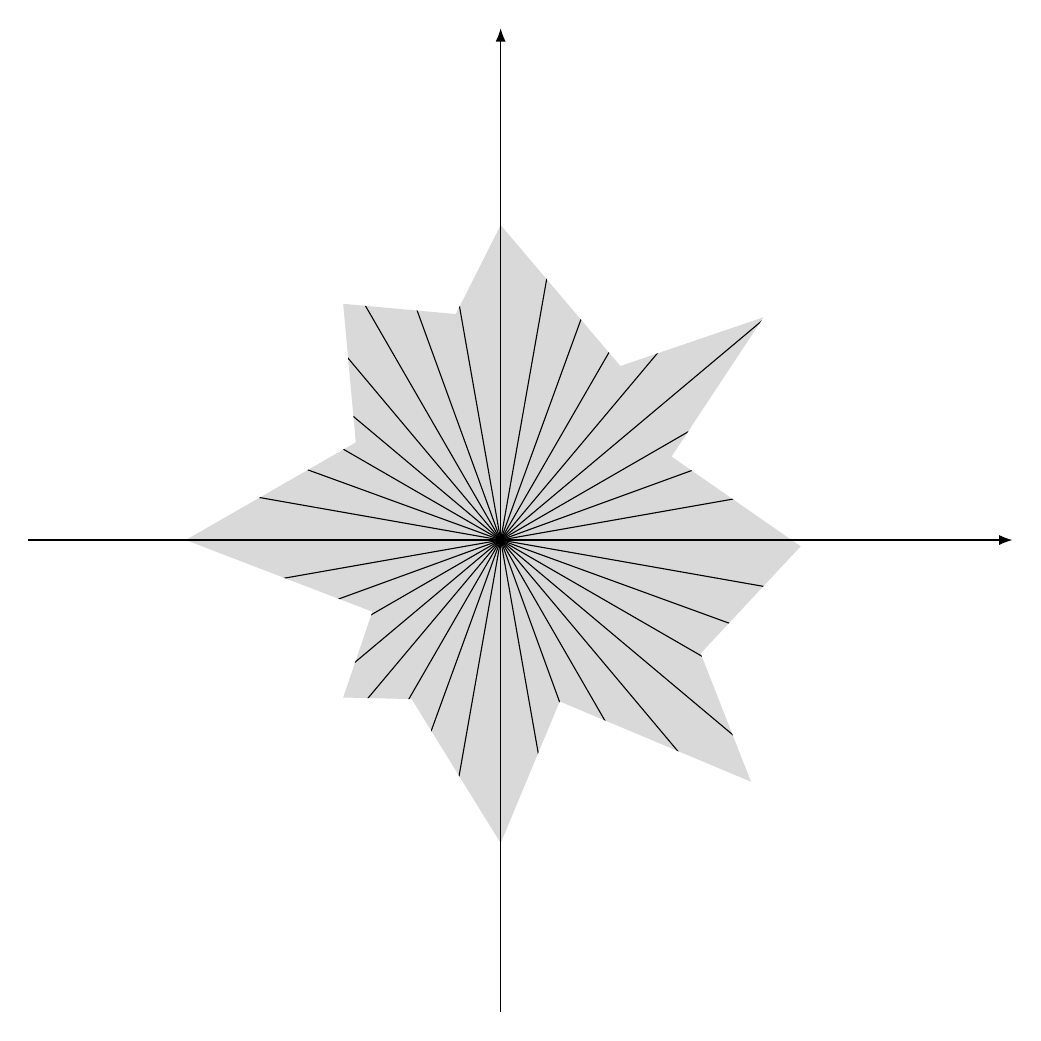
\begin{tikzpicture}
    \begin{scope}
        % clip domain
        \clip   (0, 4) -- (-0.57, 2.87) -- (-2, 3) -- (-1.84, 1.24) -- 
                (-4, 0) -- (-1.63, -0.91) -- (-2, -2) -- (-1.13, -2.02) -- 
                (0, -3.85) -- (0.75, -2.05) -- (3.18, -3.07) -- (2.54, -1.44) -- 
                (3.81, -0.08) -- (2.17, 1.06)-- (3.34, 2.83) -- (1.52, 2.21);
        \fill[gray!30] (0, 0) circle (4.42);
        % draw lines
        \foreach \theta in {0, 10, ..., 350}{
            \draw (0, 0) -- (\theta:4.42);
        } 
    \end{scope}
    % axis
    \draw[->] (-6, 0) -- (6.5, 0);
    \draw[->] (0, -6) -- (0, 6.5);
\end{tikzpicture}
\end{document}